% Created 2021-04-13 Tue 20:32
% Intended LaTeX compiler: pdflatex
\documentclass[11pt]{article}
\usepackage[utf8]{inputenc}
\usepackage[T1]{fontenc}
\usepackage{graphicx}
\usepackage{grffile}
\usepackage{longtable}
\usepackage{wrapfig}
\usepackage{rotating}
\usepackage[normalem]{ulem}
\usepackage{amsmath}
\usepackage{textcomp}
\usepackage{amssymb}
\usepackage{capt-of}
\usepackage{hyperref}
\usepackage[a4paper, lmargin=30mm, rmargin=30mm, tmargin=25mm, bmargin=25mm]{geometry}
\date{2021 April 13}
\title{TAB2XML Testing Document\\\medskip
\large For Version 1.0.0}
\hypersetup{
 pdfauthor={},
 pdftitle={TAB2XML Testing Document},
 pdfkeywords={},
 pdfsubject={},
 pdfcreator={Emacs 27.1 (Org mode 9.4.4)}, 
 pdflang={English}}
\begin{document}

\maketitle
\tableofcontents

\newpage

\section{Introduction}
\label{sec:org82f4bb6}
This document details the testing used in TAB2XML, how they were derived, how they are implemented, and why the testing is sufficient.

\begin{figure}[htbp]
\centering
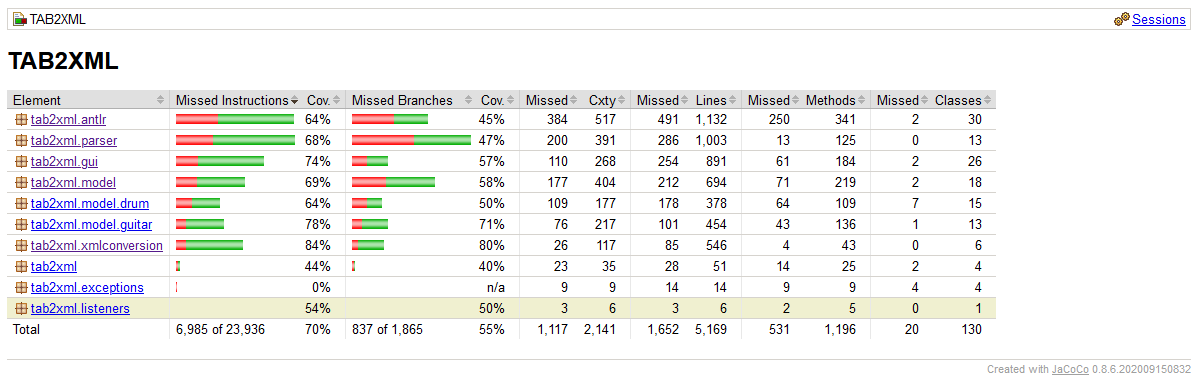
\includegraphics[width=.9\linewidth]{../Screenshots/test-coverage-20210413.png}
\caption{Test coverage report for the whole project, as of 2021-04-13.}
\end{figure}
\section{Front-End Tests}
\label{sec:org65ed0a6}
Many of the front-end tests are implemented using a \texttt{ViewBot}, a class that simulates a GUI.
\subsection{Code Coverage and Test Sufficiency}
\label{sec:org7cc92b9}
\begin{figure}[htbp]
\centering
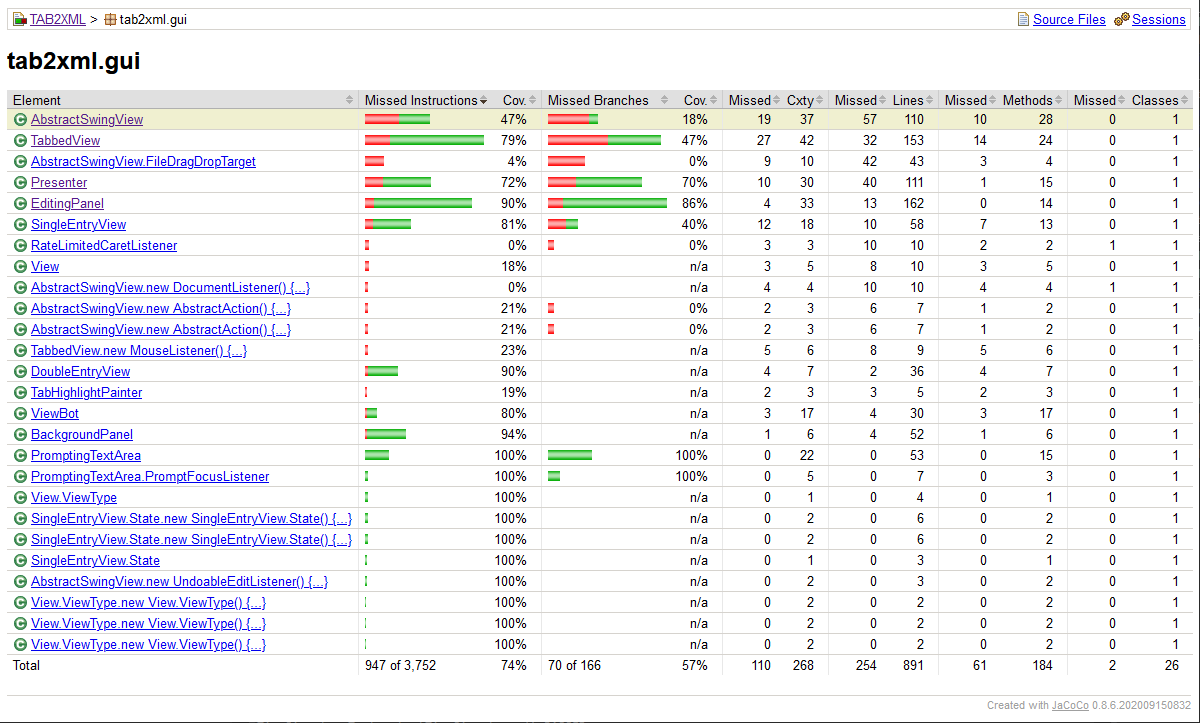
\includegraphics[width=.9\linewidth]{../Screenshots/test-coverage-20210413-gui.png}
\caption{Code coverage for the \texttt{tab2xml.gui} package, where the GUI code is located.  This report, and all statistics in the Front-End Tests section, are as of 2021-04-13.}
\end{figure}

Testing GUI code is a unique challenge, so it is unrealistic to get high code coverage of in GUI tests.  However, TAB2XML's GUI has a coverage of 74 \%, which is high for GUI tests.  All of the code not tested in \texttt{tab2xml.gui} is very hard or impossible to test automatically.  However, since almost all of these features are related to user interaction, errors can be found easily by manually running the application.  In addition, most of the uncovered code is simple enough that it may not need testing.  Much of the un-covered code involves prompting the user with a dialog box, which cannot be tested automatically.  Since each GUI functionality of TAB2XML that can be tested has a test, this testing is sufficient.
\subsection{EditingPanelTest}
\label{sec:org791b593}
This test tests the functionality of the \texttt{EditingPanel}, a custom \texttt{JPanel} that is used to edit XML metadata (by creating instances of the \texttt{XMLMetadata} class).  These test cases were derived by making one test for each important functionality of the \texttt{EditingPanel}.
\begin{itemize}
\item \texttt{testCancel()}: Tests that the "Cancel" button works properly.  It is implemented by inputting a text tab, setting a measure range, clicking Edit, editing the tab, then clicking Cancel.  The test then ensures that the input text tab was not changed.
\item \texttt{testComposer()}: Tests that the \texttt{EditingPanel} can correctly set the XMLMetadata's composer field.  It is implemented by setting the text of the panel's composer entry, then getting the panel's resulting metadata, then checking the metadata's composer field.  This is done twice: once for an empty field (the resulting metadata should have no composer) and once for a full field (the resulting metadata's composer should be the field's text).
\item \texttt{testErrors()}: Tests various situations which could cause an error, such as having a negative measure start value.  All error conditions are tested by creating the error conditions, simulating clicking a button, and using \texttt{assertThrows} or \texttt{assertDoesNotThrow} to test for an error (or no error).  Many error situations are tested.
\item \texttt{testMeasureRange1()}: Tests that empty text fields create the correct specified measure range for measure narrowing (first to last).  It is implemented by clearing the \texttt{measureStart} and \texttt{measureEnd} fields and checking the resuling measure range.
\item \texttt{testMeasureRange2()}: Tests that typing in a measure range is registered by the system.  It is implemented by setting the text of the measure range fields and then checking the resulting measure range.
\item \texttt{testNarrowing()}: Tests that the editing panel correctly calls the backend's measure narrowing functionality.  Does not test that the narrowed text is correct, as that is the job of \texttt{MeasureNarrowingTest}.  It is implemented by following a series of steps, using a \texttt{ViewBot} which is artificially connected to an \texttt{EditingPanel}:
\begin{enumerate}
\item Load a text tab into the input text area, and edit the measure fields to select a measure range
\item Ensure that the Edit button is enabled then simulate pressing it
\item Ensure that the narrowed text tab is correctly loaded into the view's narrowing text box, and that the panel registers that editing is underway
\item Use \texttt{view.setNarrowedText} to edit the narrowed text
\item Ensure that the Done button is enabled then simulate pressing it
\item Ensure that the view's input text is correctly changed, and that the panel registers that editing is complete
\end{enumerate}
\item \texttt{testTimeSignature()}: Tests that the EditingPanel correctly uses the time signature functionality.  It is implemented by setting a measure range and time signature in the EditingPanel's text fields, then simulating pressing the Set Time Signature button.  The panel's generated metadata is checked for the resulting time signature.
\item \texttt{testTitle()}: Tests that the \texttt{EditingPanel} can correctly set the title field.  It is implemented in the same way as \texttt{testComposer()}, except that the case with the empty field has a different output: the metadata should contain the default title "Untitled Score", instead of containing no title.
\end{itemize}

This testing is sufficient because every important functionality of the \texttt{EditingPanel} is tested.  The code coverage of \texttt{EditingPanel} is 90 \%.  The \texttt{XMLMetadata} class, which is related to \texttt{EditingPanel}, has 100 \% code coverage.  The only code that is not covered by tests is code that should never run, and error code that doesn't finish running due to the way the tests are implemented (because the \texttt{ViewBot}'s \texttt{showErrorMessage} method is implemented by throwing an exception, the methods are marked as missed).
\subsection{PresenterTest}
\label{sec:orgbf0f7be}
These test cases were derived by making one test for each important method of \texttt{Presenter}.
\begin{itemize}
\item \texttt{testConvert()}: Tests that the Presenter's convert method correctly interacts with the input (gets input text \& instrument, uses the parser to convert the tab and sets the output correctly).  It does not check that the converted MusicXML is correct - that is the backend tests' job.  
It is implemented by first loading a sample input from a file and converting it using the parser to get the expected output.  Then, the ViewBot simulates inputting this text and selecting the correct instrument (guitar).  Then, the presenter's convert() method is called.  Finally, the ViewBot's output text is compared with the expected output.
\item \texttt{testConvertAndSave()}: Tests that the Presenter's \texttt{convertAndSave()} method works properly.  It is basically a combination of \texttt{testConvert} and \texttt{testSaveToFile}.  In addition, it tests that the boolean argument of \texttt{convertAndSave} works properly by running twice, once per argument.
It is implemented by loading sample input and issuing a convertAndSave command, similarly to \texttt{testConvert}.  Then, both the View's output and the test file used as output have their contents checked with the correct text.  Like in \texttt{testConvert}, this output is generated by the backend code.
\item \texttt{testErrorNoSelectedFile()}: Tests that the system's commands properly fail (without halting) when the user does not select a file.  Also ensures that the system does not attempt to read from or write to any files in this situation.
It is implemented by calling the Presenter's methods before setting any file.  A simple guitar tab is put into the View's input to prevent any errors caused by the empty input.  Variables counting the number of attempts to read from and write to files is implemented in the Presenter to ensure none of these operations occur.
\item \texttt{testErrors()}: Tests that calling certain operations with an illegal state of the View correctly throws errors.
It is implemented by using the ViewBot's methods to put it in the illegal state, then executing the Presenter's methods inside a assertThrows lambda.
\item \texttt{testLoadFromFile()}: Tests that the "Load from File" command works properly.  
It is implemented by using sample text in a file.  A presenter uses its \texttt{loadFromFile()} command to load the text into a ViewBot, and the ViewBot's input text is compared with the text that was in the file.
\item \texttt{testSaveToFile()}: Tests that the "Save to File" command works properly.
Some text is put in the output of a ViewBot.  Then, a Presenter uses its \texttt{saveToFile()} command to save the text to a file.  The file's text is compared with the text that was inputted in the ViewBot.
\end{itemize}

This testing is sufficient because every method of the Presenter is covered by a test (except the constructor, which is trivial and has only one line of code).  The Presenter's methods are simple enough that only one test is necessary for each.  The Presenter has 72 \% code coverage, and most of the missed lines are trivial error handling code.
\subsection{PromptingTextAreaTest}
\label{sec:orgf22405c}
These test cases were derived by making one test case for each of the important functionalities of the \texttt{PromptingTextArea}: the colour and font of the prompt, the prompt text disappearing when the text box is focused, typing text in the box, and setting the area's font.
\begin{itemize}
\item \texttt{testAutoPromptFont()}: Tests that the PromptingTextArea correctly auto-creates prompting and non-prompting fonts.  It is implemented by setting the area's prompt font to null and then calling getPromptFont().  It expects that a newly created font is returned.
\item \texttt{testPromptColourFont()}: Tests that the text box's colour and font is set properly.  
This test works by creating a PromptingTextArea, and setting custom fonts with \texttt{setRegularFont()} and \texttt{setPromptFont()}.  The prompt is disabled, and the active colour and font is checked for correctness.  The prompt is enabled, and the same checks are performed.
\item \texttt{testPromptFocusChanges()}: Tests that the text box reacts properly to focus changes.  
This test is implemented by simulating gaining and losing focus on the text box, and testing that the text box's text updates correctly.
\item \texttt{testPromptTyping()}: Tests that the text box reacts properly to typing and when methods are run on it (setText and setPromptText).  
This test works by undergoing several operations (adding and deleting text, gaining and losing focus, changing the prompt text, manually enabling or disabling the prompt) while checking the text in the box is correct after each step.  Typing and deleting text is simulated using the setText method.
\item \texttt{testSetFont()}: Tests that fonts are set correctly.  
This test is implemented by disabling the prompt, and setting the font.  The regular, prompt and active fonts are checked for correctness.  Then, the prompt is enabled and the regular, prompt and active fonts are checked again.  The test is repeated, but the prompt starts enabled and is switched to disabled in the second step.  This is done because the setFont method behaves differently based on whether the prompt is enabled or disabled.
\end{itemize}

This testing is sufficient because every method of the PromptingTextArea is tested at least once, and all important or complex methods have tests dedicated to them and their related methods: \texttt{testPromptColourFont} tests setRegularFont() and setPromptFont(); \texttt{testPromptTyping} tests setText() and setPromptText(); \texttt{testSetFont} tests setFont().  All other public methods are simple getters or setters, or methods that trivially call one of the tested methods.  In addition, the gain or loss of focus, an important feature of the \texttt{PromptingTextArea}, has its own dedicated testing method.  The code coverage for \texttt{PromptingTextArea} is 100 \%.
\subsection{TabbedViewUserExperinceTest}
\label{sec:org555f85e}
This test tests the user experience of the default \texttt{TabbedView}.  These test cases were derived by considering the important functionality of the view.  Use cases related to metadata editing are covered by \texttt{EditingPanelTest}, so they are not tested here.
All of the tests are implemented by using the view's package-private fields to simulate the user performing a specific use case, and then checking the correctness of the values or states of the view's fields.
\begin{itemize}
\item \texttt{testConvert()}: Tests the "Convert Text Tab" use case.  The output musicXML is compared against output obtained from the backend, as testing the correctness of the output is the responsibility of the backend tests.
\item \texttt{testInputButtonState()}: Tests the state of the "Convert", "Convert and Save" and "Save Input" buttons in multiple scenarios to ensure they are correctly enabled and disabled depending on the scenario.
\item \texttt{testOutputButtonState()}: Tests the state of the "Save Output" button in multiple scenarios to ensure it is correctly enabled and disabled depending on the scenario.
\end{itemize}

This testing is sufficient because all important use cases are covered by either this test or \texttt{EditingPanelTest}.  Code coverage of the \texttt{TabbedView} class is 79 \%, and all of the missed instructions are trivial lambda instructions that do not need to be tested or things that are hard to test automatically but easy to test manually.
\subsection{TimeSignatureTest}
\label{sec:orga4592db}
This is a small test that tests the time signature setting functionality.  It was derived by thinking of situations that could cause problems, and creating one test for simple, non-problematic situations.  Both tests are implemented by creating an \texttt{XMLMetadata} instance with specific time signatures, and checking the contents of the maps returned by \texttt{getTimeSignatures()} and \texttt{getTimeSignatureRanges()}.
\begin{itemize}
\item \texttt{testTimeSignatures()}: Tests a set of time signatures where the measure ranges do not overlap.
\item \texttt{testNonDisjointIntervals()}: Tests a set of time signatures where the measure ranges do overlap.
\end{itemize}

This is sufficient testing because it tests an example of every major scenario, and test coverage for \texttt{XMLMetadata} (which has functionality other than the time signatures being tested) is 100 \%.  All instructions in \texttt{XMLMetadata} that relate to time signatures are covered by this test.
\subsection{ViewTest}
\label{sec:orgdd36d55}
These tests were derived by making one test for each major method of the View interface.

All tests in this section are run once per View supported by the program, and once for the ViewBot.  This ensures that all of the Views support every possible feature.  Any test in this section that requires use of an unimplemented optional method is skipped.  

\begin{itemize}
\item \texttt{testInputText()}: Tests that all of the standard views can correctly get and set their input text.
\item \texttt{testOutputText()}: Tests that all of the standard views can correctly get and set their output text
\item \texttt{testInstrumentSelection()}: Tests that all of the standard views can correctly get and set their instrument selection
\end{itemize}

All three of these tests are implemented by setting the parameter to some value, then comparing the value set to the value returned by the appropriate get method.

This testing is sufficient because, like in the Presenter, every important method in the View interface is tested by one test, except \texttt{showErrorMessage(String, String)}.  The showErrorMessage method cannot be tested automatically (because I do not want to specify \textbf{how} an error message is shown, only that one is shown), and it is trivial enough that I am not worried about it breaking (As of the time this document was written, all implementations of this method have only one line of code).  The View's methods are also simple enough that only one test per View is needed for each method.

\texttt{View} has 18 \% code coverage, \texttt{AbstractSwingView} has 47 \% code coverage, and the three concrete view classes each have 80-90 \% code coverage.  \texttt{View}'s code coverage is low because many of its methods are default methods that are overriden by \texttt{AbstractSwingView}, plus one static factory method that does not need to be tested.  \texttt{AbstractSwingView}'s code coverage is low because many of its methods cannot be tested automatically (though all can easily be tested manually).
\newpage

\section{Back-End Tests}
\label{sec:org8454504}

\subsection{Code Coverage and Test Sufficiency}
\label{sec:org703dd45}
Testing the Back-End is a very important part of ensuring that the system is working as intended. The coverage for the Back-End is solid overall except for areas which are either no longer used, have unimportant information, or have the testing covered by a different part of the system in their place. For example, many parts related to drums are either not used or were tested by a different part of the system since drums were implemented last, and are also simpler in comparison to guitar. The testing done for the Back-End was sufficient because many example combinations of different text tabs were tested and each example was different enough to cover all possibilities required to be converted by the system.

Code coverage reports for backend code (all as of 2021-04-13, as with all statistics in the Back-End Tests section): \\
\begin{figure}[htbp]
\centering
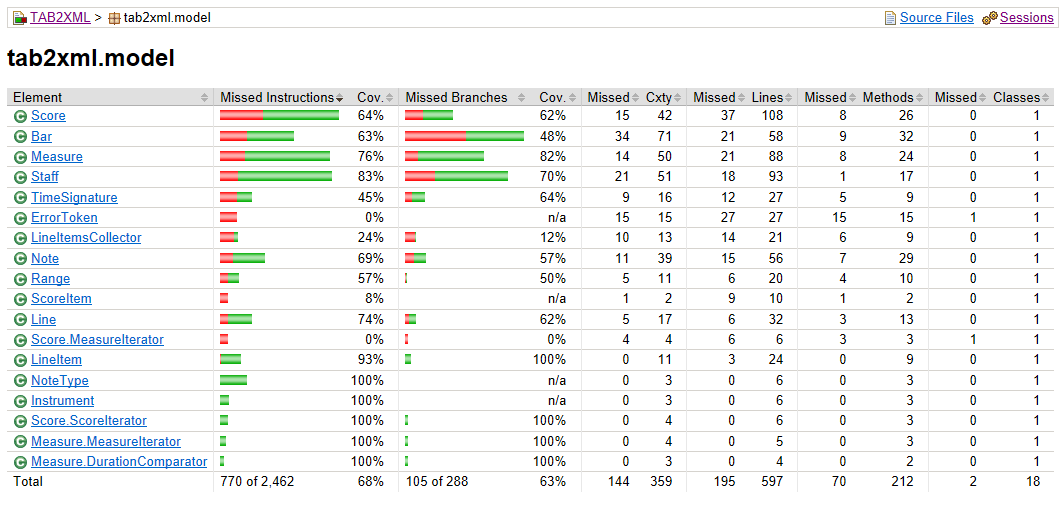
\includegraphics[width=.9\linewidth]{../Screenshots/test-coverage-20210413-model.png}
\caption{Code coverage for \texttt{tab2xml.model}}
\end{figure}
\begin{figure}[htbp]
\centering
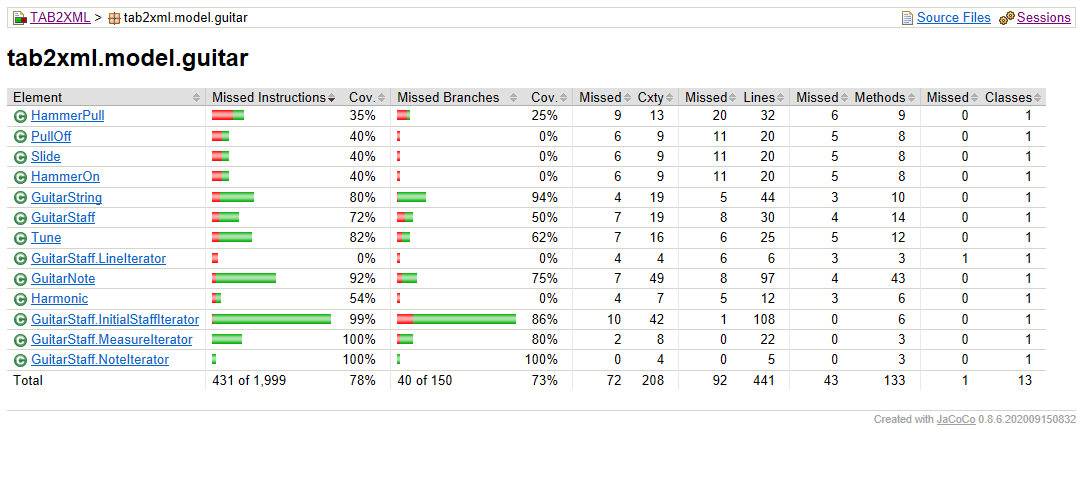
\includegraphics[width=.9\linewidth]{../Screenshots/test-coverage-20210413-model-guitar.png}
\caption{Code coverage for \texttt{tab2xml.model.guitar}}
\end{figure}
\begin{figure}[htbp]
\centering
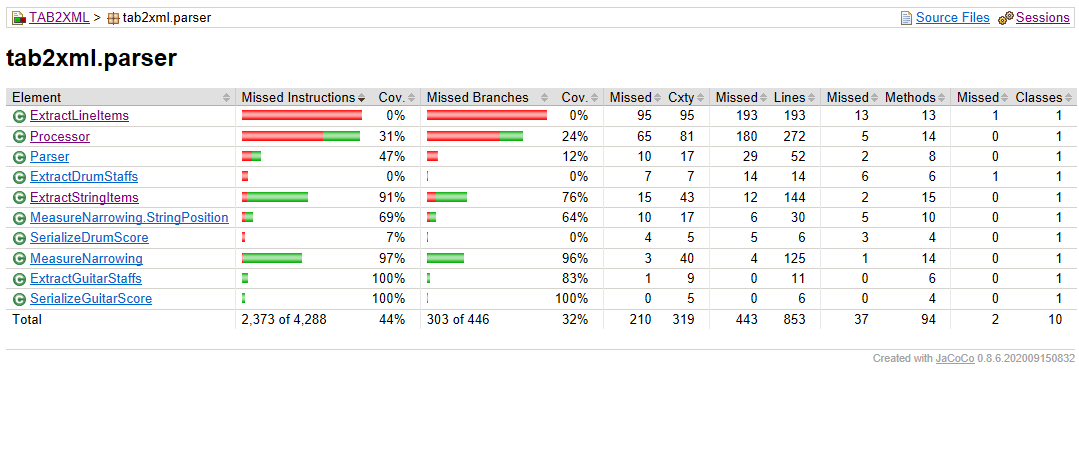
\includegraphics[width=.9\linewidth]{../Screenshots/test-coverage-20210413-parser.png}
\caption{Code coverage for \texttt{tab2xml.parser}}
\end{figure}
\begin{figure}[htbp]
\centering
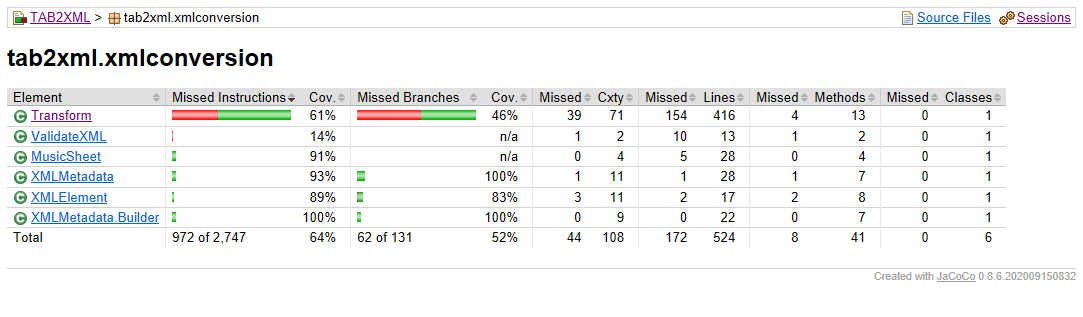
\includegraphics[width=.9\linewidth]{../Screenshots/test-coverage-20210413-xmlconversion.png}
\caption{Code coverage for \texttt{tab2xml.xmlConversion}}
\end{figure}
\subsection{ParserTest}
\label{sec:orgeb7cc4c}
These tests were derived by making sure that the parser was correctly interpreting the information provided through a text tab.
\begin{itemize}
\item \texttt{testGuitarConversion()}: Tests that Guitar conversion is handled as expected. This includes checking for the correct notes + amount of notes, correct number of strings, and correct number of measures. There is 5 versions of this test, as shown below, and each one includes different input files that handle different text tab cases.
This test was created by taking an input of a guitar tab via text file, manually recording all of the expected information in an array and comparing that expected information with the information produced by the respective functions that are used in the xml conversion process.
\item \texttt{testGuitarConversion\_0()}: This test is a simple correctness test which tests the first tablature example provided during the project. This test makes sure that the correct notes are parsed with the correct attributes.
\item \texttt{testGuitarConversion\_1()}: This test makes sure that guitar tablature with multiple staffs are parsed correctly with the correct number of measures. This will ensure that more complex tablature will be correctly parsed and in the natural order of the notes.
\item \texttt{testGuitarConversion\_2()}: This test ensures that the notes within the different guitar actions such as hammer-on are parsed correctly. This test consists of the currently supported operations for guitar excluding grace notes and repeat sections (which will be tested in the next two guitar tests).
\item \texttt{testGuitarConversion\_3()}: This test ensures that grace notes function as expected. The grace note modifier acts greedy and collects any of the notes that follow the action. This test makes sure that this attribute works together with the notes natural ordering.
\item \texttt{testGuitarConversion\_4()}: This test ensures that a basic repeat section functions as expected.
\item \texttt{testBassConversion()}: Tests that Bass conversion is handled as expected. This includes checking for the correct notes + amount of notes, correct number of strings, and correct number of measures. There is multiple versions of this test and each one includes different input files that handle different text tab cases, similar to the guitar cases above.
This test was created by taking an input of a bass tab via text file, manually recording all of the expected information in an array and comparing that expected information with the information produced by the respective functions that are used in the xml conversion process.
\item \texttt{testDrumsConversion()}: Tests that Drum conversion is handled as expected. This includes checking for the correct notes + amount of notes, correct octaves for each note, correct number of lines, and correct number of measures.
\end{itemize}
This test was created by taking an input of a drum tab via text file, manually recording all of the expected information in an array and comparing that expected information with the information produced by the respective functions that are used in the xml conversion process.
\begin{itemize}
\item \texttt{testGuitarScore()}: Tests that a guitar score object can be made successfully and have string and note objects assigned to it.
This test was created by initializing a Score object, as well as GuitarString and GuitarNote objects, and adding the former two into the Score object. The purpose of this is to make sure that these objects are correctly created as they are the core of the xml conversion process.
\item \texttt{testBassScore()}:Tests that a bass score object can be made successfully and have string and note objects assigned to it.
This test was created by initializing a Score object, as well as GuitarString and GuitarNote objects, and adding the former two into the Score object. The purpose of this is to make sure that these objects are correctly created as they are the core of the xml conversion process. Tested with the common attributes of a bass score as opposed to the test above.
\end{itemize}
This test was created by initializing a Score object, as well as GuitarString and GuitarNote objects, and adding the former two into the Score object. The purpose of this is to make sure that these objects are correctly created as they are the core of the xml conversion process.

This testing is sufficient because there are tests for each basic component of a text tab (for example, measures or strings), and ensures that the parser is able to accurately interpret and store the information. Different cases are handled by these tests to make sure that all the different types of notes are handled by the system.

\subsection{NoteTest}
\label{sec:org888a62d}
These tests were derived to make sure that note objects, which contain valuable information about notes that can be used in the xml conversion process, can be properly created. 
\begin{itemize}
\item \texttt{noteTest()}: Tests that notes have the correct name and index.
\end{itemize}
This test was created by passing note to test, expected name of note and expected index of note as the parameter.
\begin{itemize}
\item \texttt{testToNote()}: There are 2 versions of testTonote, and both of them have different arguments. The first tests the toNote method in the Note class and checks if a valid note is correctly converted, and the other one tests the invalid notes.
\end{itemize}
There are 2 testTonote. The first was created by passing the string input(\emph{"tune + fret"}) and the string this note is on, and checks if this was a valid note and if it was converted correctly by comparing it to an expected note. The 2nd one was created just by passing string input(\emph{"tune + fret"}) and checks if an invalid note was entered by using exceptions.
\begin{itemize}
\item \texttt{stringItemCompareTo()}: Tests that the parser reads the notes in the correct order that they appear in the text tab.
\end{itemize}
This test was created by hard coding an array of different notes, with different positions in the tab, and adding them to an array, then comparing each note in the array to an array of each note in the order they are expected.

This is sufficient testing because it checks that our system properly handles creating Note objects, which is a very important step in translating the information from text tabs to xml because notes are the main focus of learning songs through text tab. By testing the correctness and validity of these note objects, we can be sure that the notes that appear in a text tab will have the necessary information used in xml.

** TestArea
These tests were derived to make sure that the octaves of notes in a Guitar or Bass tab are converted correctly.
\begin{itemize}
\item \texttt{testGuitarOctaves\_0()}: Tests that guitar octaves are correct.
\end{itemize}
This test was created by calling the getOctave() method for every fret on the guitar.
\begin{itemize}
\item \texttt{testBassOctaves\_0()}: Tests that bass octaves are correct.
\end{itemize}
This test was created by calling the getOctave() method for every fret on the bass.

This is sufficient because every single fret on the instrument is tested.

\subsection{MeasureNarrowingTest}
\label{sec:org9ebeda4}
These were derived by considering the operations of \texttt{MeasureNarrowing} (including private methods) as well as the possible text tabs that could cause problems.
Each was implemented by loading a text tab from a file, then performing an operation on the loaded text tab, then checking the resulting tab against an output string.  Some tests do this twice for more confidence.

\begin{itemize}
\item \texttt{testBottomRightCorner()}: Tests the \texttt{bottomRightCorner()} private method.
\item \texttt{testDelinearize()}: Tests the \texttt{delinearize()} private method.
\item \texttt{testExtractDecoratedMeasure()}: Tests the \texttt{extractMeasureRange} method with the Capricho Arabe tab (which has a lot of extra "decoration" around its measure text)
\item \texttt{testExtractMeasure()}: Tests the \texttt{extractMeasureRange} method for a simple input (one measure at a time, one "row" of text tab)
\item \texttt{testExtractMultilineMeasure()}: Tests the \texttt{extractMeasureRange} method for a complex input (tests a multi-row text tab, extracted range goes across a row boundary)
\item \texttt{testExtractRepeatedMeasure()}: Tests the \texttt{extractMeasureRange} method on a tab with a repeated measure (since the method relies on the '|' character to delimit measures, repeated measures can cause errors by having two '|' characters).
\item \texttt{testLinearize()}: Tests the \texttt{linearize()} private method.
\item \texttt{testLinearize2()}: Tests that linearization handles blank lines at the start and end correctly.
\item \texttt{testReplaceMeasure()}: Tests the \texttt{replaceMeasureRange} method for a simple input.
\item \texttt{testReplaceMultilineMeasure()}: Tests the \texttt{replaceMeasureRange} method for a complex input.
\item \texttt{testTopLeftCorner()}: Tests the \texttt{topLeftCorner()} private method.
\end{itemize}

This is sufficent testing because multiple distinct tabs are tested, and the code coverage for \texttt{MeasureNarrowing} is 96 \%.  Its package-private static member class \texttt{StringPosition} has 69 \% code coverage, but the uncovered methods are all also unused (and all of them are trivial or autogenerated by Eclipse).
\end{document}
